\chapter{Elementi circuitali e grafi I/V}

L'analisi simbolica circuitale attinge direttamente dalla teoria dei grafi, sulla quale getta le proprie basi. Un grafo è definito come una rappresentazione astratta di un insieme di oggetti, fra i quali vi sono coppie interconnesse attraverso collegamenti diretti. Gli oggetti interconnessi vengono rappresentati con astrazioni matematiche denominate \textit{vertici}, mentre i collegamenti fra coppie di vertici vengono definiti \textit{archi}. Di norma si può dare una rappresentazione grafica di un grafo, dove i vertici vengono rappresentati come punti collegati fra loro da linee o curve, queste ultime rappresentanti gli archi.

Nel seguito verranno usati indifferentemente i termini \textit{vertice} e \textit{nodo} per fare riferimento alla stessa entità, poiché se il primo rispecchia fedelmente la teoria dei grafi, il secondo deriva direttamente dalla teoria dei circuiti.

\paragraph{}
Alla base dei metodi topologici per l'analisi e la risoluzione simbolica di circuiti elettrici vi è la sintesi di questi ultimi come coppia di grafi di corrente e tensione. I due grafi, denominati nel seguito $gI$ e $gV$, hanno alcune peculiarità importanti che, come vedremo, discendono direttamente dal processo di generazione, ovvero:
\begin{itemize}
 \item Hanno uno stesso numero di vertici $N$.
 \item Hanno uno stesso numero di archi $M$.
 \item Definiscono un ordine stretto sull'insieme degli archi.
 \item Archi corrispondenti derivano da uno stesso componente, ovvero: il $j_{esimo}$ arco di $gI$ e il $j_{esimo}$ arco di $gV$ sono inclusi nei due grafi a seguito della sintesi di uno stesso componente e non può avvenire che due archi corrispondenti facciano riferimento a due elementi diversi.
 \item Condividono informazioni fra archi corrispondenti, ovvero: il $j_{esimo}$ arco di $gI$ e il $j_{esimo}$ arco di $gV$ condividono uno stesso blocco di informazione (anche e non solo a causa del punto precedente).
\end{itemize}
Questi aspetti sono molto importanti soprattutto considerando il fatto che algoritmi come quelli che verranno discussi in seguito fanno assunzioni forti sul rispetto di determinati vincoli, quali i precedenti.

\paragraph{Grafi e circuiti}
Prima di procedere è utile fare un cenno all'argomento della sintesi di un circuito nella forma di una coppia di grafi. Un'analisi introduttiva approfondita e corredata dalle dimostrazioni necessarie la si può trovare in \cite{Percival1}, \cite{Percival2} e \cite{Percival3}. Alla base vi è l'idea che sebbene esista un metodo classico per l'analisi di circuiti basato sulle leggi di Kirchoff, questo può rappresentare per reti di grandi dimensioni un processo molto difficoltoso e irto di ostacoli, con un alto rischio di errore. Pertanto negli articoli citati, in particolare in \cite{Percival1}, è dimostrato come sia possibile innanzitutto ottenere una forma diversa a partire da un circuito, ovvero un grafo, attraverso lo studio dei suoi componenti. Tale grafo è, almeno inizialmente, usato come base per la generazione di matrici coinvolte poi nella risoluzione. Tali matrici, avendo dimensione ridotta e discendendo da una forma maggiormente compressa, permettono uno studio più accelerato. Procedendo poi viene illustrato come sia possibile risolvere il circuito, ovvero ottenere le espressioni desiderate, senza ricorrere alla trasformazione da rappresentazione topologica (grafi) ad algebrica (insiemi di equazioni, matrici e/o determinanti) \cite{Percival2}.\\
L'aspetto più interessante, però, è quello che vede il passaggio da questa forma di studio a quella che poi, attraverso modifiche e aggiustamenti, è utilizzata tutt'oggi. Infatti in \cite{Percival3} viene sfruttata la corrispondenza fra le caratteristiche topologiche ed elettriche di un circuito per dimostrare come sia possibile generare non uno, bensì una coppia di grafi (tensione e corrente) e come questa coppia di grafi sia strettamente legata alla rappresentazione algebrica. In altri termini, viene illustrato come le operazioni matriciali, che fino ad allora rappresentavano il cuore del processo di risoluzione, trovino una corrispondenza diretta $1:1$ nelle operazioni sulla coppia di grafi in corrente e tensione. Questo comporta che ogni problema risolvibile in uno dei due spazi, lo è anche nello spazio corrispondente.

Bisogna sottolineare che i processi di sintesi degli elementi in parti di grafo che nel complesso generano i due grafi in tensione e in corrente, sono componente integrante di questo lavoro, poiché nei processi risolutivi vengono sfruttate proprio tali rappresentazioni. Allo stesso tempo, però, esula dagli scopi una discussione e spiegazione approfondita sul perché tali processi di sintesi possano avere luogo, poiché la complessità e pesantezza delle dimostrazioni risulterebbe fuori luogo e non potrebbe in alcun modo aiutare a comprendere meglio quelli che sono, invece, gli argomenti cardine discussi. Si rimanda ancora una volta agli articoli in \cite{Percival1}, \cite{Percival2} e \cite{Percival3} per i necessari approfondimenti.

\paragraph{}

\begin{table}[b]
 \centering
 \begin{tabular}[h]{|c|i|c|i|}
  \toprule
   \textbf{Elemento} & \textbf{Simbolo} & \multicolumn{2}{|c|}{\textbf{Rappresentazione}} \\
  \midrule
    \multirow{2}{*}{R , G} & \multirow{2}{*}{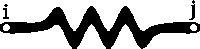
\includegraphics[scale=0.6]{immagini/resistor.pdf}} & gI & 
\includegraphics[scale=0.9]{immagini/ijedge.pdf}\\
    & & gV & 
\includegraphics[scale=0.9]{immagini/jiedge.pdf} \\
  \midrule
    \multirow{2}{*}{C} & \multirow{2}{*}{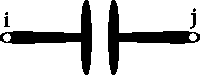
\includegraphics[scale=0.6]{immagini/capacitor.pdf}} & gI & 
\includegraphics[scale=0.9]{immagini/ijedge.pdf}\\
    & & gV & 
\includegraphics[scale=0.9]{immagini/jiedge.pdf} \\
  \midrule
    \multirow{2}{*}{L} & \multirow{2}{*}{
\includegraphics[scale=0.6]{immagini/inductor.pdf}} & gI & 
\includegraphics[scale=0.9]{immagini/ijedge.pdf}\\
    & & gV & 
\includegraphics[scale=0.9]{immagini/jiedge.pdf} \\
 \bottomrule
 \end{tabular}
 \caption{Rappresentazione componenti}
 \label{tab:basecmp}
\end{table}

I modelli adottati nel lavoro di tesi e qui discussi sono gli stessi che già in precedenza sono stati sfruttati in seno al progetto riguardante l'analisi simbolica per l'Università degli Studi di Firenze. Nella tabella \ref{tab:basecmp} sono riportate graficamente le relazioni fra componenti base e grafi in tensione e in corrente di un circuito.\graffito{Ricordiamo che il grafo è pesato e una stessa rappresentazione in termini di archi differisce in realtà per quanto riguarda etichetta, valore e grado associati} Bisogna notare che la rappresentazione di questi elementi è praticamente immediata e consiste in un solo arco posto tra i due nodi, in entrambi i grafi. Vedremo come questo sia in realtà il caso più semplice nella migrazione da circuito a coppia di grafi e quali complicazioni riservino altre categorie di componenti.

\paragraph{Nullatore, noratore e nullore}

\begin{figure}[b]
 \centering
 \subfloat[Nullatore]{\label{fig:nullator}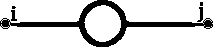
\includegraphics[scale=0.75]{immagini/nullator.pdf}}\hspace{25pt}
 \subfloat[Noratore]{\label{fig:norator}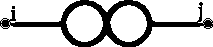
\includegraphics[scale=0.75]{immagini/norator.pdf}}\\
 \subfloat[Nullore]{\label{fig:nullor}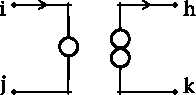
\includegraphics[scale=1]{immagini/nullor.pdf}}
 \caption{Nullatore, noratore e nullore}
 \label{fig:nullorcmp}
\end{figure}

Ancora prima di parlare degli altri componenti, è utile introdurre due elementi che aiuteranno nella comprensione di quanto segue, ovvero il nullatore e il noratore, oltre alla loro diretta estensione, il nullore, osservabili in figura \ref{fig:nullorcmp}.\\
Il nullatore, figura \ref{fig:nullator}, è descritto da \cite{Wikipedia} come:
\begin{quote}
 Un bipolo teorico lineare tempo invariante definito da una corrente e una tensione nulle ai propri capi. Presenta contemporaneamente le proprietà di un corto circuito (tensione nulla) e di un circuito aperto (corrente nulla). Non si comporta né come generatore di corrente né come generatore di tensione, sebbene sia entrambi allo stesso tempo. L'inserimento di un nullatore in un circuito schematico impone vincoli matematici sul comportamento di quest'ultimo, forzando il circuito stesso ad adottare qualsiasi comportamento possibile per far fronte alle richieste. Per esempio l'ingresso di un amplificatore operazionale si comporta come un nullatore, poiché non presenta né assorbimento di corrente né tensione fra i due terminali.
\end{quote}
Il noratore, figura \ref{fig:norator}, è descritto da \cite{Wikipedia} come:
\begin{quote}
 Un bipolo teorico lineare tempo invariante definito da una corrente e una tensione arbitrari ai propri capi. Un noratore rappresenta un generatore controllato di tensione o di corrente con guadagno infinito. L'inserimento di un noratore in un circuito schematico fornisce corrente e tensione a qualsiasi componente esterno le richieda. Per esempio l'uscita di un amplificatore operazionale si comporta come un noratore, producendo tensioni e correnti che soddisfano le richieste del circuito a valle, a discapito di un ingresso nullo.
\end{quote}
Entrambi i componenti se presi singolarmente rappresentano elementi privi di significato. Sono solitamente utilizzati in stretta associazione l'uno con l'altro per definire elementi composti più complessi. Combinandoli in parallelo si ottiene il bipolo corto circuito, mentre la combinazione in serie da luogo ad un bipolo circuito aperto. L'uso più comune è però quello della combinazione come quadripolo (rete 2-porte) ideale, ovvero il nullore riportato in figura \ref{fig:nullor}, dove vengono posti un nullatore in ingresso e un noratore in uscita. Il nullore rappresenta un amplificatore ideale con guadagni di corrente, tensione, transconduttanza e transimpedenza infiniti, i cui parametri di trasmissione possono essere riassunti nella forma matriciale che segue:
$$
\left(
 \begin{array}{c}
  V_{in} \\ I_{in}
 \end{array}
\right)
=
\left(
 \begin{array}{cc}
  0 & 0 \\ 0 & 0
 \end{array}
\right)
\left(
 \begin{array}{c}
  V_{out} \\ I_{out}
 \end{array}
\right)
$$
Per la sua struttura intrinseca e a causa delle imposizioni dettate da nullatore e noratore, il nullore non assorbe corrente e non sussite alcuna differenza di potenziale ai suoi capi. Fra i due terminali sono imposte alcune condizioni sul comportamento, forzando lo schema a far sì che le relazioni costitutive presenti fra loro siano rispettate. Questo lo si può riassumere nella sintesi sotto forma di grafo in corrente e in tensione come segue:
\begin{itemize}
 \item I due nodi ai capi del nullatore collassano nel grafo in tensione.
 \item I due nodi ai capi del noratore collassano nel grafo in corrente.
\end{itemize}
Poiché quanto sopra non è evidentemente possibile (i due nodi sono e devono restare distinti, anche all'interno della coppia di grafi), si forza la presenza dei rami relativi al componente in ognuno degli alberi comuni fra i grafi in corrente e in tensione.\graffito{Il collasso fra vertici può essere simulato forzando un arco fittizio che li unisca negli alberi di copertura, poiché questo preclude la presenza negli alberi stessi di ogni altro arco presente fra i due vertici} In altri termini l'algoritmo di ricerca degli alberi comuni, trattato in seguito, dovrà forzare preventivamente in essi la presenza dei rami nullatore per il grafo in tensione e dei rami noratore per il grafo in corrente, di fatto definendo una radice comune per ogni albero che verrà a formarsi. 

\begin{figure}[b]
 \centering
 \subfloat[A.O.]{\label{fig:ao}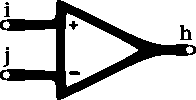
\includegraphics{immagini/opampl.pdf}}\\
 \subfloat[G.I.]{\label{fig:aogi}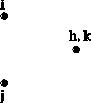
\includegraphics{immagini/nullorgi.pdf}}\hspace{50pt}
 \subfloat[G.V.]{\label{fig:aogv}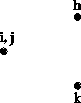
\includegraphics{immagini/nullorgv.pdf}}
 \caption{Rappresentazione di un amplificatore operazionale}
 \label{fig:aocmp}
\end{figure}

In figura \ref{fig:aocmp} è illustrata graficamente la gestione di un amplificatore operazionale ideale (\ref{fig:ao}) nella sintesi sotto forma di grafo in corrente (\ref{fig:aogi}) e grafo in tensione (\ref{fig:aogv}). Se ne ricava un componente costituito, come introdotto in precedenza, da una coppia nullatore-noratore (nullore) dislocati rispettivamente fra i nodi $i$, $j$, $h$ e massa (che sostituisce di fatto il vertice $k$). Concludendo con la parentesi su questa tipologia di componenti particolari basti sapere che, come verrà illustrato in seguito, il nullore è strettamente coinvolto nella rappresentazione non solo dell'amplificatore operazionale ma anche di gran parte dei generatori controllati.

\paragraph{Generatori controllati e non}

\begin{figure}[t]
 \centering
 \subfloat[VCCS]{\label{fig:vccs}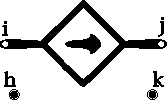
\includegraphics{immagini/vccs.pdf}}\\
 \subfloat[G.I.]{\label{fig:vccsgi}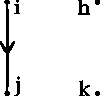
\includegraphics{immagini/vccsgi.pdf}}\hspace{50pt}
 \subfloat[G.V.]{\label{fig:vccsgv}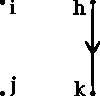
\includegraphics{immagini/vccsgv.pdf}}
 \caption{Generatore di corrente controllato in tensione}
 \label{fig:vccscmp}
\end{figure}

Leggermente più complessa la sintesi dei generatori controllati.\\
La forma più semplice è data dal generatore di corrente controllato in tensione\graffito{Generatore di corrente controllato in tension o VCCS (Voltage Controlled Current Source)}, in figura \ref{fig:vccs}, a causa della sua equazione costitutiva. Come si può osservare, il contributo apportato consiste nell'aggiunta di un arco fra i nodi d'ingresso (\ref{fig:vccsgv}) nel grafo in tensione e un arco fra i terminali d'uscita nel grafo in corrente (\ref{fig:vccsgi}). Per inciso questo è l'unico generatore controllato sintetizzato direttamente, poiché negli altri casi si è dovuti ricorrere a modelli alternativi per riuscire a sposare le richieste degli algoritmi a valle.

\begin{figure}[b]
 \centering
 \subfloat[CCVS]{\label{fig:ccvs}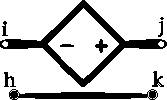
\includegraphics{immagini/ccvs.pdf}}\\
 \subfloat[Circuito equivalente]{\label{fig:ccvseq}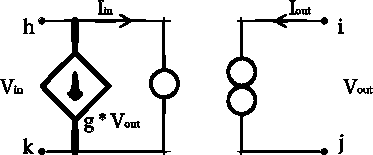
\includegraphics{immagini/ccvseq.pdf}}
 \caption{Generatore di tensione controllato in corrente}
 \label{fig:ccvscmp}
\end{figure}

In figura \ref{fig:ccvscmp} è riportato un generatore di tensione controllato in corrente\graffito{Generatore di tensione controllato in corrente o CCVS (Current Controlled Voltage Source)} (\ref{fig:ccvs}) ed il suo modello equivalente (\ref{fig:ccvseq}), realizzato con i componenti visti precedentemente. Non viene riportata, poiché intuibile, la rappresentazione in forma di grafo in corrente e grafo in tensione, sebbene essa sia direttamente ricavabile da quanto detto a proposito del generatore di corrente controllato in tensione e del nullore. Più precisamente, il generatore di tensione controllato in corrente vedrà:
\begin{itemize}
 \item un arco nel grafo in tensione fra i nodi $h$ e $k$ e uno fra $i$ e $j$ nel grafo in corrente, dovuti al nullore (che, ricordiamo, dovranno essere forzati in ogni albero comune).
 \item un arco nel grafo in tensione fra i nodi $i$ e $j$ e uno fra $h$ e $k$ nel grafo in corrente, dovuti al generatore di corrente controllato in tensione.
\end{itemize}
La relazione costitutiva del modello equivalente risulta essere:
$$ V_{out} = \frac{V_{in}}{g};\quad I_ {in} = 0; $$

\begin{figure}[t]
 \centering
 \subfloat[VCVS]{\label{fig:vcvs}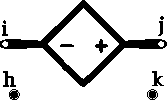
\includegraphics{immagini/vcvs.pdf}}\\
 \subfloat[Circuito equivalente]{\label{fig:vcvseq}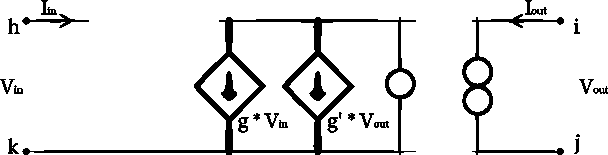
\includegraphics{immagini/vcvseq.pdf}}
 \caption{Generatore di tensione controllato in tensione}
 \label{fig:vcvscmp}
\end{figure}

Discretamente più complesso il modello equivalente del generatore di tensione controllato in tensione\graffito{Generatore di tensione controllato in tensione o VCVS (Voltage Controlled Voltage Source)}, riportato in figura \ref{fig:vcvscmp}. Per la rappresentazione scelta, infatti, si ha la necessità di coinvolgere un nodo ulteriore (oltre ai quattro terminali di ingresso/uscita) dove saranno agganciati i due generatori controllati ed il nullatore. Posto che sia $l$ l'etichetta di tale nodo, in questo caso avremo, a seconda dei componenti coinvolti:
\begin{itemize}
 \item un arco nel grafo in tensione fra i nodi $h$ e $k$ e uno fra $i$ e $j$ nel grafo in corrente, dovuti al nullore (che, ricordiamo, dovranno essere forzati in ogni albero comune).
 \item un arco nel grafo in tensione fra i nodi $i$ e $j$ e uno fra $l$ e $k$ nel grafo in corrente, dovuti ad uno dei due generatori di corrente controllati in tensione.
 \item un arco nel grafo in tensione fra i nodi $h$ e $k$ e uno fra $l$ e $k$ nel grafo in corrente, dovuti al secondo dei due generatori controllati.
\end{itemize}
La relazione costitutiva del modello equivalente risulta essere:
$$ V_{out} = -\frac{g}{g'}\ast V_{in};\quad I_ {in} = 0; $$

\begin{figure}[b]
 \centering
 \subfloat[CCCS]{\label{fig:cccs}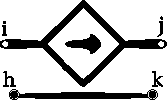
\includegraphics{immagini/cccs.pdf}}\\
 \subfloat[Circuito equivalente]{\label{fig:cccseq}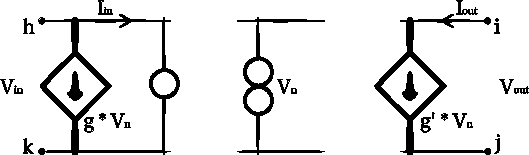
\includegraphics{immagini/cccseq.pdf}}
 \caption{Generatore di corrente controllato in corrente}
 \label{fig:cccscmp}
\end{figure}

Altrettanto complesso il modello equivalente del generatore di corrente controllato in corrente\graffito{Generatore di corrente controllato in corrente o CCCS (Current Controlled Current Source)}, riportato in figura \ref{fig:cccscmp}. Anche in questo caso, come già per il componente visto in precedenza, si ha la necessità di sfruttare un nodo fittizio al quale verrà agganciato il noratore. Posto anche stavolta che sia $l$ tale nodo, avremo:
\begin{itemize}
 \item un arco nel grafo in tensione fra i nodi $h$ e $k$ e uno fra $l$ e $k$ nel grafo in corrente, dovuti al nullore (che, ricordiamo, dovranno essere forzati in ogni albero comune).
 \item un arco nel grafo in tensione fra i nodi $l$ e $k$ e uno fra $h$ e $k$ nel grafo in corrente, dovuti ad uno dei due generatori di corrente controllati in tensione.
 \item un arco nel grafo in tensione fra i nodi $l$ e $k$ e uno fra $i$ e $j$ nel grafo in corrente, dovuti al secondo dei due generatori controllati.
\end{itemize}
La relazione costitutiva del modello equivalente risulta essere:
$$ I_{out} = -\frac{g}{g'}\ast I_{in};\quad V_ {in} = 0; $$

Può forse sembrare fuorviante complicare la rappresentazione di elementi di per sé rappresentabili in modi più sintetici, sotto forma di grafo in corrente e in tensione. In letteratura, infatti, non mancano modelli alternativi che non coinvolgano così tanti componenti. Ciò nonostante va detto che quanto sopra descritto, rappresentato nei diversi modelli equivalenti, si adatta perfettamente alle necessità dell'algoritmo per la ricerca degli alberi comuni a valle del processo di sintesi. Il numero di archi inseriti nei due diversi grafi relativi al circuito, cioè grafo in tensione e grafo in corrente, è infatti lo stesso e tali archi sono sempre dislocati a gruppi fra stessi insiemi di terminali; se ne deduce che i due grafi avranno infine uno stesso numero di nodi e di archi. Questa condizione è, come spiegato in seguito, alla base del funzionamento dell'algoritmo di ricerca degli alberi comuni fra due grafi. Anche la richiesta di terminali ulteriori, fittizi è limitata e non conduce in alcun caso a discostamenti dalle condizioni citate.

\paragraph{}

\begin{figure}[b]
 \centering
 \subfloat[Generatore di tensione]{\label{fig:vgen}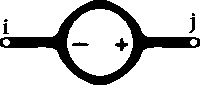
\includegraphics{immagini/voltage.pdf}}\hspace{50pt}
 \subfloat[Generatore di corrente]{\label{fig:igen}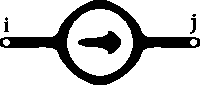
\includegraphics{immagini/current.pdf}}
 \caption{Generatori}
 \label{fig:gens}
\end{figure}

Dall'analisi appena effettuata sembrano mancare due dei componenti più importanti, ovvero i generatori di tensione (figura \ref{fig:vgen}) e i generatori di corrente (figura \ref{fig:igen}). Per quanto riguarda la loro inclusione all'interno del processo di sintesi, è stato scelto un approccio particolare. L'idea alla base è quella di inserire all'interno di ogni singolo circuito un generatore fittizio i cui parametri, opportunamente fissati, non influenzino in alcun modo eventuali generatori da esso controllati. In altri termini il generatore fittizio (per essere precisi, un generatore di tensione)\graffito{Un procedimento simile può essere applicato adottando come riferimento anche un generatore di corrente} è tale per cui, ad esempio, le correnti e le tensioni dei generatori controllati da esso possono essere definite semplicemente attraverso un'oculata politica di assegnazione dei parametri di controllo. Questo fa sì che non vi sia più bisogno di trovare un modello diretto o indiretto per la rappresentazione dei generatori di corrente e di tensione, bensì basterà renderli intelligentemente controllati dal generatore fittizio.\\
Consideriamo per esempio di voler inserire nel circuito un generatore di tensione $V$, questo lo si renderà direttamente controllato dal generatore di tensione fittizio $V_f$. Otteniamo un generatore di tensione controllato in tensione, che sappiamo come trattare, con la necessità di impostare opportunamente i parametri. Supponendo una tensione per $V_f$ pari a $1$ (dalla figura \ref{fig:vcvs}, $V_{in} = 1$), basterà porre $g'$ pari a $-1$ e $g$ pari al valore che si intende assegnare a $V$, ottenendo così quanto desiderato da:
$$ V = -\frac{g}{g'}\ast V_{f};$$
Intuitivamente, questo trucco ha un prezzo da pagare. Il rovescio della medaglia è la necessità di ulteriori terminali fra cui porre il generatore fittizio (ovvero almeno un terminale) col conseguente aumento di complessità per la gestione di generatori di corrente e di tensione non controllati come generatori controllati. Questo si traduce in una lieve crescita nella dimensione dei due grafi in corrente e in tensione associati al circuito, e quindi in un maggiore sforzo computazionale per la risoluzione.

\paragraph{}

\begin{figure}
 \centering
 \subfloat[Modello]{\label{fig:transformer}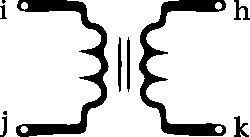
\includegraphics{immagini/transformer.pdf}}\hspace{50pt}
 \subfloat[Circuito equivalente]{\label{fig:transeq}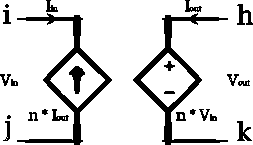
\includegraphics{immagini/transformereq.pdf}}
 \caption{Rappresentazione di un trasformatore ideale}
 \label{fig:trans}
\end{figure}

Proseguendo nella carrellata sui componenti disponibili per il disegno schematico e in particolare su quelli creati a partire dai generatori controllati, in figura \ref{fig:trans} sono riportati componente e circuito equivalente relativi ad un trasformatore ideale. Nel caso specifico ci si ricollega al modello generale, valido a prescindere, del trasformatore ideale, composto appunto da due generatori controllati incrociati (un generatore di corrente controllato in corrente ed un generatore di tensione controllato in tensione), ovvero tali da far sì che i terminali di controllo del primo rappresentino i terminali di uscita del secondo e viceversa. Anche in questo caso, a parte alcuni accorgimenti specifici a livello di programmazione, utili a rendere effettivamente sensibile il componente alla corrente di controllo (si ha la necessità di un nodo fittizio di corredo), si è aggiunto un nuovo elemento sfruttando esclusivamente ciò di cui già disponevamo, alleggerendo il tutto tanto a livello teorico quanto pratico.

\begin{figure}
 \centering
 \subfloat[Modello]{\label{fig:mutualinductance}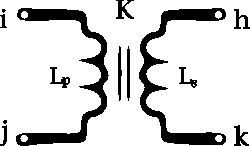
\includegraphics{immagini/mutualinductance.pdf}}\\\vspace{25pt}
 \subfloat[Circuito equivalente]{\label{fig:mutindeq}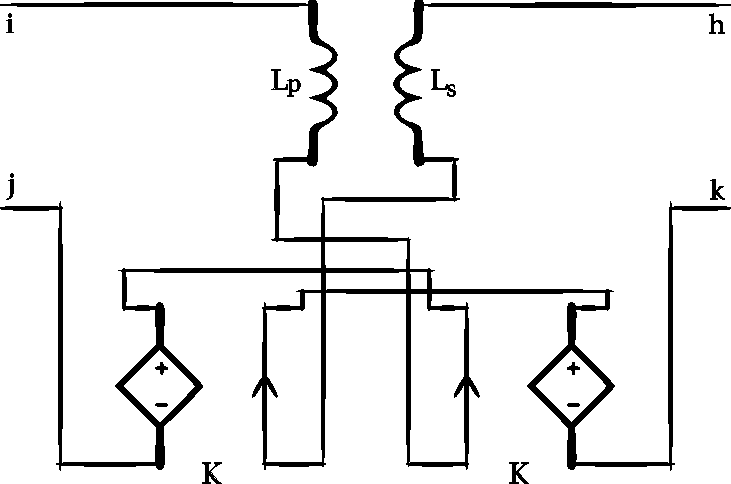
\includegraphics[scale=0.65]{immagini/mutualinductanceeq.pdf}}
 \caption{Rappresentazione di una mutua induttanza}
 \label{fig:mutind}
\end{figure}

Un procedimento simile, sviluppato attraverso l'aggiunta di nodi fittizi e altri piccoli accorgimenti a livello software, riguarda la mutua induttanza (riportata in figura \ref{fig:mutind} e in forma simbolica in \ref{fig:mutualinductance}). In questo caso si fa uso di generatori di tensione controllati in corrente accoppiati con induttori e si ha la necessità di ben quattro nodi fittizi. Ancora più importante, nell'esempio, il fatto che per un corretto funzionamento bisogna agire aggirando la corretta modalità di apporto dei dati da parte dei generatori controllati, forzando per essi un grado pari a $1$ per la variabile libera $s$ (sarebbe normalmente $0$). Questo è necessario poiché essi vanno a sostituire quello che sarebbe un altro induttore nel modello passivo alternativo e concorrono, nello schema equivalente in figura \ref{fig:mutindeq}, a mettere in relazione fra loro i due induttori componenti della mutua induttanza.

\paragraph{Conclusione}
Attraverso quanto illustrato nei paragrafi precedenti si è visto come, attraverso quelli che sono pochi oggetti elementari quali resistenze, ammettenze o nullori, si riescano a comporre elementi ben più complessi come ad esempio i generatori controllati. A partire da questi, inoltre, si sono realizzati ulteriori componenti come composizione di elementi aggregati, il che rende fede all'idea che attraverso questa tecnica tutto ciò che è modellabile con gli oggetti base è di fatto realizzabile in termini di grafi equivalenti. Pertanto, sebbene non risultino direttamente realizzabili elementi quali ad esempio i transistori, ne sono perfettamente modellabili i loro circuiti equivalenti come quello per piccoli segnali. Questo dovrebbe far intuire la flessibilità e la capacità espressiva di uno strumento in grado di dar luogo all'analisi simbolica, basti pensare infatti che attraverso di esso si possono potenzialmente analizzare tutti quei circuiti che sono esprimibili come modelli equivalenti contenenti gli elementi base accettati dal sistema.
